\documentclass[10pt,letterpaper,final,twoside,notitlepage]{article}
\usepackage[margin=.5in]{geometry} % 1/2 inch margins on all pages
\usepackage[utf8]{inputenc} % Define the input encoding
\usepackage[USenglish]{babel} % Define language used
\usepackage{amsmath,amsfonts,amssymb}
\usepackage{amsthm} % Gives us plain, definition, and remark to use in \theoremstyle{style}
\usepackage{mathtools} % Allow for text and math in align* environment.
\usepackage{thmtools}
\usepackage{thm-restate}
\usepackage{graphicx}

\usepackage[
backend=biber,
style=alphabetic,
citestyle=authoryear]{biblatex} % Must include citation somewhere in document to print bibliography
\usepackage{hyperref} % Generate hyperlinks to referenced items
\usepackage[nottoc]{tocbibind} % Prints the Reference/Bibliography in TOC as well
\usepackage[noabbrev,nameinlink]{cleveref} % Fancy cross-references in the document everywhere
\usepackage{nameref} % Can make references by name to places
\usepackage{caption} % Allows for greater control over captions in figure, algorithm, table, etc. environments
\usepackage{subcaption} % Allows for multiple figures in one Figure environment
\usepackage[binary-units=true]{siunitx} % Gives us ways to typeset units for stuff
\usepackage{csquotes} % Context-sensitive quotation facilities
\usepackage{enumitem} % Provides [noitemsep, nolistsep] for more compact lists
\usepackage{chngcntr} % Allows us to tamper with the counter a little more
\usepackage{empheq} % Allow boxing of equations in special math environments
\usepackage[x11names]{xcolor} % Gives access to coloring text in environments or just text, MUST be before tikz
\usepackage{tcolorbox} % Allows us to create boxes of various types for examples
\usepackage{tikz} % Allows us to create TikZ and PGF Pictures
\usepackage{ctable} % Greater control over tables and how they look
\usepackage{diagbox} % Allow us to have shared diagonal cells in tables
\usepackage{multirow} % Allow us to have a single cell in a table span multiple rows
\usepackage{titling} % Put document information throughout the document programmatically
\usepackage[linesnumbered,ruled,vlined]{algorithm2e} % Allows us to write algorithms in a nice style.

\counterwithin{figure}{section}
\counterwithin{table}{section}
\counterwithin{equation}{section}
\counterwithin{algocf}{section}
\crefname{algocf}{algorithm}{algorithms}
\Crefname{algocf}{Algorithm}{Algorithms}
\setcounter{secnumdepth}{4}
\setcounter{tocdepth}{4} % Include \paragraph in toc
\crefname{paragraph}{paragraph}{paragraphs}
\Crefname{paragraph}{Paragraph}{Paragraphs}

% Create a theorem environment
\theoremstyle{plain}
\newtheorem{theorem}{Theorem}[section]
% Create a numbered theorem-like environment for lemmas
\newtheorem{lemma}{Lemma}[theorem]

% Create a definition environment
\theoremstyle{definition}
\newtheorem{definition}{Defn}
\newtheorem{corollary}{Corollary}[section]
% \begin{definition}[Term] \label{def:}
%   Make sure the term is emphasized with \emph{term}.
%   This ensures that if \emph is changed, it shows up everywhere
% \end{definition}

% Create a numbered remark environment numbered based on definition
% NOTE: This version of remark MUST go inside a definition environment
\theoremstyle{remark}
\newtheorem{remark}{Remark}[definition]
%\counterwithin{definition}{subsection} % Uncomment to have definitions use section.subsection numbering

% Create an unnumbered remark environment for general use
% NOTE: This version of remark has NO restrictions on placement
\newtheorem*{remark*}{Remark}

% Create a special list that handles properties. It can be broken and restarted
\newlist{propertylist}{enumerate}{1} % {Name}{Template}{Max Depth}
% [newlistname, LevelsToApplyTo]{formatting options}
\setlist[propertylist, 1]{label=\textbf{(\roman*)}, ref=\textbf{(\roman*)}, noitemsep, nolistsep}
\crefname{propertylisti}{property}{properties}
\Crefname{propertylisti}{Property}{Properties}

% Create a special list that handles enumerate starting with lower letters. Breakable/Restartable.
\newlist{boldalphlist}{enumerate}{1} % {Name}{Template}{Max Depth}
% [newlistname, LevelsToApplyTo]{formatting options}
\setlist[boldalphlist, 1]{label=\textbf{(\alph*)}, ref=\alph*, noitemsep, nolistsep} % Set options

\newlist{nocrefenumerate}{enumerate}{1} % {Name}{Template}{Max Depth}
% [newlistname, LevelsToApplyTo]{formatting options}
\setlist[nocrefenumerate, 1]{label=(\arabic*), ref=(\arabic*), noitemsep, nolistsep}

% Create a list that allows for deeper nesting of numbers. By default enumerate only allows depth=4.
\newlist{nestednums}{enumerate}{6}
% [newlistname, LevelsToApplyTo]{formatting options}
\setlist[nestednums]{noitemsep, label*=\arabic*.}

\tcbuselibrary{breakable} % Allow tcolorboxes to be broken across pages
% Create a tcolorbox for examples
% /begin{example}[extra name]{NAME}
% Create a tcolorbox for examples
% Argument #1 is optional, given by [], that is the textbook's problem number
% Argument #2 is mandatory, given by {}, that is the title for the example
% Avoid putting special characters, (), [], {}, ",", etc. in the title.
\newtcolorbox[auto counter,
number within=section,
number format=\arabic,
crefname={example}{examples}, % Define reference format for cref (No Capitals)
Crefname={Example}{Examples}, % Reference format for cleveref (With Capitals)
]{example}[2][]{ % The [2][] Means the first argument is optional
  width=\textwidth,
  title={Example \thetcbcounter: #2. #1}, % Parentheses and commas are not well supported
  fonttitle=\bfseries,
  label={ex:#2},
  nameref=#2,
  colbacktitle=white!100!black,
  coltitle=black!100!white,
  colback=white!100!black,
  upperbox=visible,
  lowerbox=visible,
  sharp corners=all,
  breakable
}

% Create a tcolorbox for general use
\newtcolorbox[% auto counter,
% number within=section,
% number format=\arabic,
% crefname={example}{examples}, % Define reference format for cref (No Capitals)
% Crefname={Example}{Examples}, % Reference format for cleveref (With Capitals)
]{blackbox}{
  width=\textwidth,
  % title={},
  fonttitle=\bfseries,
  % label={},
  % nameref=,
  colbacktitle=white!100!black,
  coltitle=black!100!white,
  colback=white!100!black,
  upperbox=visible,
  lowerbox=visible,
  sharp corners=all
}

% Redefine the 'end of proof' symbol to be a black square, not blank
\renewcommand{\qedsymbol}{$\blacksquare$} % Change proofs to have black square at end

% Common Mathematical Stuff
\newcommand{\Abs}[1]{\ensuremath{\lvert #1 \rvert}}
\newcommand{\DNE}{\ensuremath{\mathrm{DNE}}} % Used when limit of function Does Not Exist

% Complex Numbers functions
\renewcommand{\Re}{\operatorname{Re}} % Redefine to use the command, but not the fraktur version
\renewcommand{\Im}{\operatorname{Im}} % Redefine to use the command, but not the fraktur version
\newcommand{\Real}[1]{\ensuremath{\Re \lbrace #1 \rbrace}}
\newcommand{\Imag}[1]{\ensuremath{\Im \lbrace #1 \rbrace}}
\newcommand{\Conjugate}[1]{\ensuremath{\overline{#1}}}
\newcommand{\Modulus}[1]{\ensuremath{\lvert #1 \rvert}}
\DeclareMathOperator{\PrincipalArg}{\ensuremath{Arg}}

% Math Operators that are useful to abstract the written math away to one spot
% Number Sets
\DeclareMathOperator{\RealNumbers}{\ensuremath{\mathbb{R}}}
\DeclareMathOperator{\AllIntegers}{\ensuremath{\mathbb{Z}}}
\DeclareMathOperator{\PositiveInts}{\ensuremath{\mathbb{Z}^{+}}}
\DeclareMathOperator{\NegativeInts}{\ensuremath{\mathbb{Z}^{-}}}
\DeclareMathOperator{\NaturalNumbers}{\ensuremath{\mathbb{N}}}
\DeclareMathOperator{\ComplexNumbers}{\ensuremath{\mathbb{C}}}
\DeclareMathOperator{\RationalNumbers}{\ensuremath{\mathbb{Q}}}

% Calculus operators
\DeclareMathOperator*{\argmax}{argmax} % Thin Space and subscripts are UNDER in display

% Signal and System Functions
\DeclareMathOperator{\UnitStep}{\mathcal{U}}
\DeclareMathOperator{\sinc}{sinc} % sinc(x) = (sin(pi x)/(pi x))

% Transformations
\DeclareMathOperator{\Lapl}{\mathcal{L}} % Declare a Laplace symbol to be used

% Logical Operators
\DeclareMathOperator{\XOR}{\oplus}

% x86 CPU Registers
\newcommand{\rbpRegister}{\texttt{\%rbp}}
\newcommand{\rspRegister}{\texttt{\%rsp}}
\newcommand{\ripRegister}{\texttt{\%rip}}
\newcommand{\raxRegister}{\texttt{\%rax}}
\newcommand{\rbxRegister}{\texttt{\%rbx}}

%%% Local Variables:
%%% mode: latex
%%% TeX-master: shared
%%% End:


% These packages are more specific to certain documents, but will be availabe in the template
% \usepackage{esint} % Provides us with more types of integral symbols to use
% \usepackage[outputdir=./TeX_Output]{minted} % Allow us to nicely typeset 300+ programming languages
% This document must be compiled with the -shell-escape flag if the packages above are uncommented

\graphicspath{{./Drawings/EITP20-Secure_Systems_Engineering}} % Uncomment this to use pictures in this document
% \addbibresource{./Bibliographies/CourseNum-Name.bib}

% Math Operators that are useful to abstract the written math away to one spot
% These are supposed to be document-specific mathematical operators that will make life easier
% Many fundamental operators are defined in Reference_Sheet_Preamble.tex

\begin{titlepage}
  \title{EITP20: Secure Systems Engineering --- Final Exam Study Questions}
  \author{Karl Hallsby}
  \date{Last Edited: \today} % We want to inform people when this document was last edited
\end{titlepage}

\begin{document}
\pagenumbering{gobble}
\maketitle
\pagenumbering{roman} % i, ii, iii on beginning pages, that don't have content
\tableofcontents
\clearpage
\pagenumbering{arabic} % 1,2,3 on content pages

\section{Design Process}\label{sec:Design_Process}
\begin{questions}
\question{} Which are the steps involved in the overall design process of a secure system?
  \begin{solution}
    \begin{enumerate}[noitemsep]
    \item Threat Analysis
    \item Security Requirements
    \item \nameref{sec:Security_Architectures}
    \item \nameref{sec:Security_Design}
    \item \nameref{sec:Security_Evaluation}
    \end{enumerate}
  \end{solution}

  \begin{parts}
  \part{} Describe the relationship between the different steps?
    \begin{solution}
      In the Threat Analysis, the system is first scoped, to ensure that we limit our possibilities a little bit.
      Then, we attempt to find potential threats to the scoped system by performing one or more techniques (``Attacker can steal sensitive personal information.'').

      Once we find the potential threats, we use those along with any information/requirements given by the client to develop Security Requirements (``We require the use of encryption on personal data.'').

      The Security Architecture is the phase where we determine the kind of infrastructure we will need, the communication flows that are possible, find the interactions in the system, etc.
      This allows us to place our requirements onto the system as it exists already, and allow us to design for the system AND its longevity (``The personal info server is kept physically separate from others, only only communicates over mutually authenticated means using an appropriate cryptographic key.'').

      The Security Design is the process of actually choosing the standard, protocols, and hardware used to build the system (``The server will use keys generated by a Hardware Security Module, to ensure randomness.'').

      The Security Evaluation is done by going back to the Security Requirements and comparing the solutions you built in the Security Design and flows you developed in the Security Architecture to see if the requirements were satisfied.
      Other considerations can be put here too, including business ones (``Using a too difficult encryption algorithm will cause slowdowns of data requests/uses of the personal information.'').
    \end{solution}
  \end{parts}

\question{} In which way does a use-case description assist in the secure system design process?
  \begin{solution}
    It gives a general idea of \emph{how} the system will be used.
    This is important, because you can design a secure system in multiple ways to counter multiple threats.
    But, given the use-case of the client, there may be restrictions on what you can design for.
    It will help you derive the Security Requirements for the system, helping you Architect, Design, and Evaluate later in the process.
  \end{solution}

\question{} What is a threat analysis?
  \begin{solution}
    The process of finding potential threats to a system.
    These can be from inside the client's group, outside, or anywhere else.
    Using one or more methods, the applier can find current vulnerabilities, and future problems with the system.
    These are used after being given the use-case description, so that potential attack vectors can be limited to some extent.
  \end{solution}

\question{} What is the main purpose of performing a threat analysis?
  \begin{solution}
    It helps find the potential vulnerabilities in a system that \textbf{HAVE NOT} been found already.
    This will give a broader overview of the system, allowing for a more general, and hopefully, more all-encompassing secure system design.
  \end{solution}

\question{} Can you give examples of threat analysis approaches?
  \begin{solution}
    \begin{enumerate}[noitemsep]
    \item Schneier Attack Trees
    \item Microsoft's STRIDE Analysis
      \begin{enumerate}[noitemsep]
      \item Spoofing
      \item Tampering
      \item Repudiation
      \item Information Disclosure
      \item Denial of Service
      \item Elevation of Privilege
      \end{enumerate}
    \item MITRE's TARA Analysis
      \begin{enumerate}[noitemsep]
      \item Crown Jewel Analysis
      \item Cyber Risk Remediation Analysis
      \item Cyber Threat Susceptability Analysis
      \end{enumerate}
    \end{enumerate}
  \end{solution}

\question{} What is the purpose of a security requirements list?
  \begin{solution}
    To ensure that you (the secure system designer) and the stakeholders/clients/users of your system design can agree on what must be done.
    Agreement here will ensure the system is secure from both perspectives and that all parites are on the same page when it comes to the issue of security.
  \end{solution}

  \begin{parts}
  \part{} Can you list input sources for deriving security requirements?
    \begin{solution}
      \begin{itemize}[noitemsep]
      \item The use-case description.
      \item The client's system needs.
      \item The client's limitations on cost and performance.
      \item The results from the threat analysis.
      \item Further discussions and interaction between the designer and the client.
      \end{itemize}
    \end{solution}

  \part{} Which are the duties of the security engineering in the security requirements gathering process?
  \end{parts}

\question{} Can you elaborate on the main differences between security requirements and other system requirements?
\question{} Please list at least three different “types” of security architectures?
  \begin{parts}
  \part{} Explain the main differences between the different listed types?
  \end{parts}

\question{} Which are the main steps preceeding the actual secuirty design step?
\question{} Explain the main design choices that need to be done at the security design process.
\question{} List and explain different type of security evaluations that typically are done ”in house”
\question{} List and explain different type of security evaluations that typically are done by external experts
\question{} What is a pen test and what is the purpose of such test?
\question{} What is a protocol analysis tool and what is the purpose of using such tool?
\question{} What is the Common Criteria (CC) standard?
  \begin{parts}
  \part{} List the 7 evaluation levels defined in CC and explain the main differences between the levels?
  \part{} List the three different system documents part of a CC and describe their main purpose.
  \end{parts}

\question{} What is CISSP?\@
\end{questions}

%%% Local Variables:
%%% mode: latex
%%% TeX-master: "../EITP20-Secure_Systems_Engineering-Study_Questions"
%%% End:


\section{Threat Analysis and Security Requirements}\label{sec:Threat_Analysis-Security_Requirements}
\begin{questions}
\question{} List three different typical security threats to an IT system?
\question{} What is the first step in an attack tree threat analysis process?
\question{} Make an attack tree based analysis of a BankID system
\question{} List three well established threat assessment methodologies
\question{} Spell out the acronym STRIDE
  \begin{parts}
  \part{} Explain the meaning of the six different concepts in STRIDE
  \part{} Give examples of attacks for the six different concepts in STRIDE
  \end{parts}

\question{} Which are the three basic steps in STRIDE?\@
\question{} Which are the two main activities in a MITRE TARA security analysis
  \begin{parts}
  \part{} Which are the main input sources to these two analysis
    activities?
  \part{} The output of these two activities are stored in special databases. What is the name of these two databases?
  \end{parts}

\question{} Describe briefly the different steps performed during a TARA CTSA
\question{} Spell out the acronyms CAPEC, CWE and CVE
  \begin{parts}
  \part{} What does CAPEC contain and how it is used in a TARA analysis?
  \part{} What does CWE contain and how it is used in a TARA analysis?
  \part{} What does CVE contain and how it is used in a TARA analysis?
  \end{parts}

\question{} Describe briefly the different steps performed during a TARA CRRA
\question{} Where can one find TTP mitigation solutions?
\question{} Which are the four different mitigation types?
\question{} Which are the steps used to obtain a final ranking table for countermeasures?
\question{} How do one select final TARA recommendations based on a countermeasure ranking table?
\question{} Which are the three mandatory parts of a TARA TTP recommendation?
\question{} Which are the different input sources to the security requirements derivation process?
\question{} Which are the main outputs from the attack tree, the STRIDE and the TARA process respectively which are used to derive high-level security requirements?
\question{} Give example of high level security requirements for a Bank ID system
\question{} Give example of low level security requirements  for a Bank ID system
\question{} Describe a four step approach for security requirements identification and documentation
\end{questions}

%%% Local Variables:
%%% mode: latex
%%% TeX-master: "../EITP20-Secure_Systems_Engineering-Study_Questions"
%%% End:


\section{Security Architectures}\label{sec:Security_Architectures}
\begin{questions}
\question{} Describe what constitutes a security architecture and give some examples.
  \begin{solution}
    A Security Architecture has graphical and textual representations of a security system.
    It includes relations, trust levels, trust relationships, and interfaces between different parts of the system.
    It also has security and system boundaries to delimit different parts of the system that have various properties.
  \end{solution}

\question{} The Sherwood Applied Business Security Architecture (SABSA) consist of 5 layers and one cross layer.
  \begin{parts}
  \part{} Describe the different layer views and list the names of the different layers.
    \begin{solution}
      \begin{enumerate}[noitemsep]
      \item Contextual Security Architecture is the view the business has of the system.
        It is quite similar to the Security Requirements.
      \item Conceptual Security Architecture is the highest-level view that an engineer can have of the system.
        This includes the general breakdown into secure portions of a system.
      \item Logical Security Architecture is the next level, that deals with data and its logical flows.
        Here, the way that data and its logical propagation are safeguarded is first developed.
      \item Physical Security Architecture is the 3rd design level.
        Here, the specific high-level security requirements and previous security architecture levels are combined to choose what needs to be done to secure the data.
      \item Component Security Architecture is the lowest level of the SABSA Security Architecture.
        Here, the actual protocols, standards, and hardware are chosen.
      \item Security Service Management Architecture is the ``cross layer''.
        It is concerned with how to maintain the system and its security.
      \end{enumerate}
    \end{solution}

  \part{} Give examples of questions the different SABSA architecture views are supposed to answer.
    \begin{solution}
      \begin{enumerate}[noitemsep]
      \item Contextual Security Architecture
        \begin{itemize}[noitemsep]
        \item What does the business need from the system?
        \item Why do we need to mitigate against these risks and threats?
        \item How do we protect the processes in this system?
        \item Who are going to be the ones using the system?
        \item Where is this system going to be geographically located and where is this product going to be used?
        \item When does the client require this system and for how long?
        \end{itemize}
      \item Conceptual Security Architecture
        \begin{itemize}[noitemsep]
        \item What does the client need to have protected?
        \item Why are these risks that need to be mitigated and do these assets need protection?
        \item How do we provide protection, in very high-level technical and maanagement security terms/strategies?
        \item Who are the people/organizations involved in the security management and the assumed trust relationships?
        \item Where is protection needed in terms of security domains?
        \item When is the relevant time scope(s) of the system's protection?
        \end{itemize}
      \item Logical Security Architecture
        \begin{itemize}[noitemsep]
        \item What is the actual information being secured?
        \item Why shall this security policy be applied to the system?
        \item How are the actual security services in the system put together?
        \item Who are the entities in the system and how can they interact?
        \item Where are the security domains and the relationships between the domains?
        \item When is the security processing cycle?
        \end{itemize}
      \item Physical Security Architecture
        \begin{itemize}[noitemsep]
        \item What is the data model and security-related data structures?
        \item Why are these the rules that drive logical decisions in the system?
        \item How do these security mechanisms work to provice security and what physical machines or modules are needed?
        \item Who are the users, the applications they use, and the security interface?
        \item Where is the required security infrastructure required to provide the security?
        \item When is the dependency in the system present in the form of execution control structures?
        \end{itemize}
      \item Component Security Architecture
        \begin{itemize}[noitemsep]
        \item What are the data field specifications, address specifications, etc.
        \item Why are we using these security standards and best practices?
        \item How are the entities/modules, tools, etc.\ used and put together?
        \item Who are the users' identities, privileges, functions, actions, Access Control Lists?
        \item Where are the computing processes, nodes addresses, and inter-process protocols?
        \item When are the security step timings and sequencing?
        \end{itemize}
      \item Security Service Management Architecture
        \begin{itemize}[noitemsep]
        \item What is the operational continuity and information processing of the system?
        \item Why do we need to minimize operational risks and mitigate failures/disruptions?
        \item How do we perform these specialized security-related operations?
        \item Who do we support? All users and their applications?
        \item Where do we perform maintainance from and on?
        \item When do we schedule things and execute our time-table of security-related operations?
        \end{itemize}
      \end{enumerate}
    \end{solution}
  \end{parts}

\question{} Which are the three different types of security services in a logical security architecture?
  \begin{solution}
    \begin{enumerate}[noitemsep]
    \item Prevention services
    \item Detection, Notification, Assurance, and Event Collection services
    \item Recovery and Restoration services
    \end{enumerate}
  \end{solution}

  \begin{parts}
  \part{} List and explain examples of services part of the non-prevention type of security services.
    \begin{solution}
      \begin{itemize}[noitemsep]
      \item Detection, Notification, Assurance, and Event Collection services
        \begin{itemize}[noitemsep]
        \item Log review
        \item Message integrity verification
        \item Security monitoring
        \item Audit trails
        \item Security Training/awareness
        \item Intrusion Detection
        \end{itemize}
      \item Recovery and Restoration services
        \begin{itemize}[noitemsep]
        \item Incident response
        \item Data replication
        \item Data backup
        \item Disaster recovery
        \item Crisis management
        \end{itemize}
      \end{itemize}
    \end{solution}
  \end{parts}

\question{} Describe each of the different prevention security services in more details.
  \begin{parts}
  \part{} Give example of at least four different communication security services and how they contribute to security prevention.
  \part{} Give example of at least four different application level security services and how they contribute to security prevention.
  \part{} Give example of at least four security management services and how they contribute to security prevention.
  \part{} Give example of at least four different Entity Security Services and how they contribute to security prevention.
    \begin{solution}
      \begin{enumerate}[noitemsep]
      \item Unique Entity naming
      \item Entity registration
      \item Entity credentials certifications
      \item Directory services
      \item Entity authorization
      \item User authentication
      \item Device authentication
      \end{enumerate}
    \end{solution}

  \end{parts}

\item Draw a picture showing the relations between major different security services from a systems point of view.
\item A logical security architecture can be created using a six steps methodology:
  \begin{parts}
  \part{} Describe each of the different steps
  \part{} What is the end result?
  \part{} Give an example of a logical security architecture
  \end{parts}

\item What is a physical security architecture?
\item A physical security architecture when using the SABSA include making a mapping to physical security mechanisms
  \begin{parts}
  \part{} Describe what is meant by a ``Naming and registration'' mechanism and give examples
  \part{} Describe what is meant by a ``Storage and runtime'' mechanism and give examples
  \part{} Describe what is meant by a ``Physical security'' mechanism and give examples
  \part{} Describe what is meant by an ``Authentication and session'' protection mechanism and give examples
  \part{} Describe what is meant by a ``User interface and naming'' mechanism and give examples
  \part{} Describe what is meant by a ``Authorization and access control'' mechanism and give examples
  \part{} Describe what is meant by a ``Monitoring and incident'' mechanism and give examples
  \end{parts}

\item What must in addition to the security mechanisms be specified in the physical security architecture?
\item Give example of platform security solution that can be used to build solutions meeting a logical security services and can be used to protect the chosen physical security mechanism?
\item For the SSO logical security architecture given at the lecture, perform the following:
  \begin{parts}
  \part{} Identify the main physical security mechanisms needed in the corresponding physical security architecture.
  \part{} Identify the main platform security components needed to fulfil the architecture
    \begin{subparts}
    \subpart{} Suggest concrete platform security mechanisms to use for the physical realization.
    \end{subparts}
  \end{parts}
\end{questions}

%%% Local Variables:
%%% mode: latex
%%% TeX-master: "../EITP20-Secure_Systems_Engineering-Study_Questions"
%%% End:


\section{Security Design}\label{sec:Security_Design}
\begin{questions}
\question{} Can you list four different principles upon which a security design should be based?
  \begin{solution}
    \begin{enumerate}[noitemsep]
    \item Use well-proven techniques, standards, libraries, hardware modules, and solutions.
    \item Keep system complexity as low as possible.
    \item Minimize the utilization of trusted components.
    \item Only develop your own solutions when really needed.
    \item Use open designs whenever possible.
    \end{enumerate}
  \end{solution}

  \begin{parts}
  \part{} Give a motivation for each of the listed design principles
    \begin{solution}
      \begin{enumerate}[noitemsep]
      \item Well-proven solutions are constantly tested, so they have more verification of their security.
      \item By reducing the number of things that can go wrong, the system can be more secure.
        The reduced number of vulnerabilities means we can focus more on the ones that remain.
      \item The greater the reliance on trusted components, the more trust that must be placed in the hardware of the system.
      \item Developing novel and unique solutions requires a lot of design and engineering time. Additionally, if they are not well-designed, they can cause more problems than they solve.
      \item By using open designs, there is a lower risk of licensing issues.
      \end{enumerate}
    \end{solution}
  \end{parts}

\question{} Describe the process steps to perform when going from a security architecture to a design specification.
  \begin{solution}
    \begin{enumerate}[noitemsep]
    \item Start with the Security Architecture.
    \item Map the desired security services to security standards.
    \item Identify gaps that are present in the System Design/Architecture.
      \begin{itemize}[noitemsep]
      \item Complement the existing Security Design/Architecture with new Designs if needed.
      \end{itemize}
    \item Perform a \nameref{sec:Security_Evaluation}.
    \item Document the \nameref{sec:Security_Design}.
    \item Identify implementation efforts (missing hardware/software).
    \end{enumerate}
  \end{solution}

\question{} What is typically the role of unique identities in security systems?
  \begin{solution}
    To create a unique mapping from name to key, allowing for reliable authentication.
    This unique name can be used for discrete access control and authorization decisions in the system.
  \end{solution}

  \begin{parts}
  \part{} Give example of three different widely used identity types?
    \begin{solution}
      \begin{enumerate}[noitemsep]
      \item ITU
      \item IEEE's MAC Addresses
      \item IETF and URIs
      \end{enumerate}
    \end{solution}
  \end{parts}

\question{} What is the problem from privacy perspective with using fixed identities?
  \begin{solution}
    If the identity has been compromised (on the back-end), it can be traced back to a user/device.
  \end{solution}

  \begin{parts}
  \part{} Describe two different methods for avoiding the identity privacy problem in a system design
    \begin{solution}
      \begin{enumerate}[noitemsep]
      \item Randomly Generated Pseudonym.
        There is a middle-man that receives the unique identifier and assigns a random value to that, which is changed each time, and allows for identification of that user/device for that session.
      \item Encrypted Identity that is not visible outside trusted container boundaries.
      \end{enumerate}
    \end{solution}
  \end{parts}

\question{} What is a digital certificate and how it is used?
  \begin{solution}
    A digital certificate is a way to securely distribute cryptographic keys while ensuring that they come from the correct person.
  \end{solution}

  \begin{parts}
  \part{} Which are the most important data fields in an X.509 certificate?
    \begin{solution}
      \begin{itemize}[noitemsep]
      \item The algorithm used in the signature
      \item The Certificate Issuer's name
      \item The period of validity
      \item The Receipient's public key information
      \end{itemize}
    \end{solution}
  \end{parts}

\question{} Which is the most used authentication principle over HTTP?\@
  \begin{solution}
    The most common priniciple is the Challenge principle.
    The only way that the correct user can authenticate with the service is by solving a challenge only the real user should know.
  \end{solution}

  \begin{parts}
  \part{} Under which circumstances can basic authentication be used
  \part{} How are typically basic authentication treated at the server side and what is the main reason for using this type of storage?
  \part{} Describe the different steps in an HTTP basic authentication.
    \begin{solution}
      \begin{enumerate}[noitemsep]
      \item The client performs a \texttt{GET} request.
      \item The server responds with \texttt{Error 401: Unauthorized}, which asks the user to input information.
      \item The client returns their credentials.
      \item The server checks their credentials.
      \item The server either returns \texttt{Error 200: OK} or \texttt{Error 403: Forbidden}.
      \end{enumerate}
    \end{solution}

  \end{parts}

\question{} Describe the principles behind hardware token based authentication
\question{} What is the rationale behind two factor authentication?
\question{} What are the main differences between:
  \begin{parts}
  \part{} TLS server authentication
  \part{} TLS client certificate authentication
  \part{} TLS pre-share key authentication
  \end{parts}

\question{} Explain the main principle behind an object security scheme
  \begin{parts}
  \part{} How does it differs from a session protection scheme like TLS or IPsec?
  \end{parts}

\question{} What does RBAC and ABAC stand for with respect to access control systems?
  \begin{parts}
  \part{} Explain the main differences between RBAC and ABAC
  \end{parts}

\question{} What is the purpose with an access token?
  \begin{parts}
  \part{} What does a SAML assertion contain?
  \end{parts}

\question{} How can a Hardware Security Module (HSM) assist in protection of cloud data storage?
\question{} List a couple of widely used commercial server anti-virus tools
\question{} How can the security of a Docker container be enhanced beyond using default configurations?
\question{} How can a Web design be made to make ``clickjacking'' less likely?
\question{} What is the main difference between key provisioning of a public key system compare to a symmetric key-based systems?
  \begin{parts}
  \part{} What are the key issues to consider when making a public key issuing design?
  \part{} Which are the key issues to consider when making a symmetric key issuing design?
  \end{parts}

\question{} List the three main different intrusion detection principles and explain how they work on high level
\question{} What is syslog and how is it typically used?
\question{} What is the main risks with a debug interface (like JTAG) and how should it be treated in a product design to avoid these risks?
\question{} Which are the three different most severe attacks threats against smart card designs and which are the typical countermeasures?
\question{} Give three examples of widely used NIST security standards and what they specify?
\question{} What does IETF stand for?
  \begin{parts}
  \part{} Give example of two well-knows IETF security standards and explain what they specify?
  \end{parts}

\question{} Which type of security standards are done by IEEE and 3GPP respectively?
\question{} What is the difference between public industry bodies and industry standards?
\question{} What is meant by a cancellable biometric protection scheme?
  \begin{parts}
  \part{} Describe how to achieve a cancellable biometric matching system
  \part{} Which alternative biometrics protection approaches can be used?
  \end{parts}
\end{questions}

%%% Local Variables:
%%% mode: latex
%%% TeX-master: "../EITP20-Secure_Systems_Engineering-Study_Questions"
%%% End:


\section{Security Evaluation}\label{sec:Security_Evaluation}
\begin{questions}
\question{} What is the purpose with a security review and when should it be performed?
  \begin{solution}
    A security review is intended to perform a general ``sanity'' check that the chosen Security Architecture makes sense.
    It also helps identify potential gaps in the Security Architecture that might have been missed.
    It can also provide a business evaluation of the chosen architecture to find business consequences.
    Lastly, we take the perspective of an attacker attempting to break into the system.

    Generally, this is done after the Architecture and Design is completed, but performing it regularly during these steps also works.
  \end{solution}

\question{} At which four main levels do you typically perform a security evaluation?
  \begin{solution}
    \begin{enumerate}[noitemsep]
    \item Security Architecture Review
    \item Design against Requirements Review
    \item Design Review
    \item Implementation Review
    \end{enumerate}
  \end{solution}

  \begin{parts}
  \part{} At which occasion should they be done?
    \begin{solution}
      \begin{enumerate}[noitemsep]
      \item After the Security Architecture design selections.
      \item Before the Security Design Specification.
      \item After the Security Design Specification.
      \item Before the system's release.
      \end{enumerate}
    \end{solution}
  \end{parts}

\question{} Mention three different aspects to consider at an architecture ``sanity check'' review.
  \begin{solution}
    \begin{enumerate}[noitemsep]
    \item System purpose vs. Security
    \item Usability Check
    \item Administrative Burden
    \end{enumerate}
  \end{solution}

  \begin{parts}
  \part{} For each aspect, list what should be considered?
    \begin{solution}
      \begin{enumerate}[noitemsep]
      \item
        \begin{itemize}[noitemsep]
        \item Does the chosen Security Architecture change any system functions?
        \item Are the security functions adding any new system properties?
        \item Can these new security functions be accepted the end-users?
        \end{itemize}
      \item
        \begin{itemize}[noitemsep]
        \item Will the security functions have any direct usability considerations?
        \item If they do, are they acceptable?
        \item Is it possible to modify the system to make it easier to use while maintaining security?
        \end{itemize}
      \item
        \begin{itemize}[noitemsep]
        \item Which routines and security policies are necessary to make the architecture functional?
        \item How costly is it to maintain the routines and policies?
        \item How much will the system be dependent on manual routines?
        \end{itemize}
      \end{enumerate}
    \end{solution}
  \end{parts}

\question{} Mention three different aspects to consider at an architecture business review.
  \begin{solution}
    \begin{enumerate}[noitemsep]
    \item Security Control
    \item Customer Relations
    \item Business Risks and Opportunities
    \end{enumerate}
  \end{solution}

  \begin{parts}
  \part{} For each aspect, list what should be considered?
  \end{parts}

\question{} What do you perform during a security requirements review?
\question{} Mention four different aspects to consider at a design review
  \begin{parts}
  \part{} For each aspect, list what should be considered?
  \end{parts}

\question{} Describe a process for issuing and security testing of a software product
  \begin{parts}
  \part{} What is the role in the process for the security officer, the security architect, the security master and security penetration tester respectively?
  \end{parts}

\question{} Give examples of things to consider during a performance review of a design?

\question{} What is the purpose of trying to ``measure'' the security of a design?
\question{} A simple security measurement takes three basic security characteristics into account:
  \begin{parts}
  \part{} Which three characteristics are then measured and how to you combine the measurements to get an overall measurement of a system?
  \end{parts}

\question{} Consider the smart card security system in \Cref{fig:Smart_Card_Security_System}.
  Assume the side-channel and physical channel break are equal important and the overall smart card security is the minmum strength of the two nodes.
  Calculate the smart card security score using the weighted weakest link approach.
  \begin{figure}[h!]
    \centering
    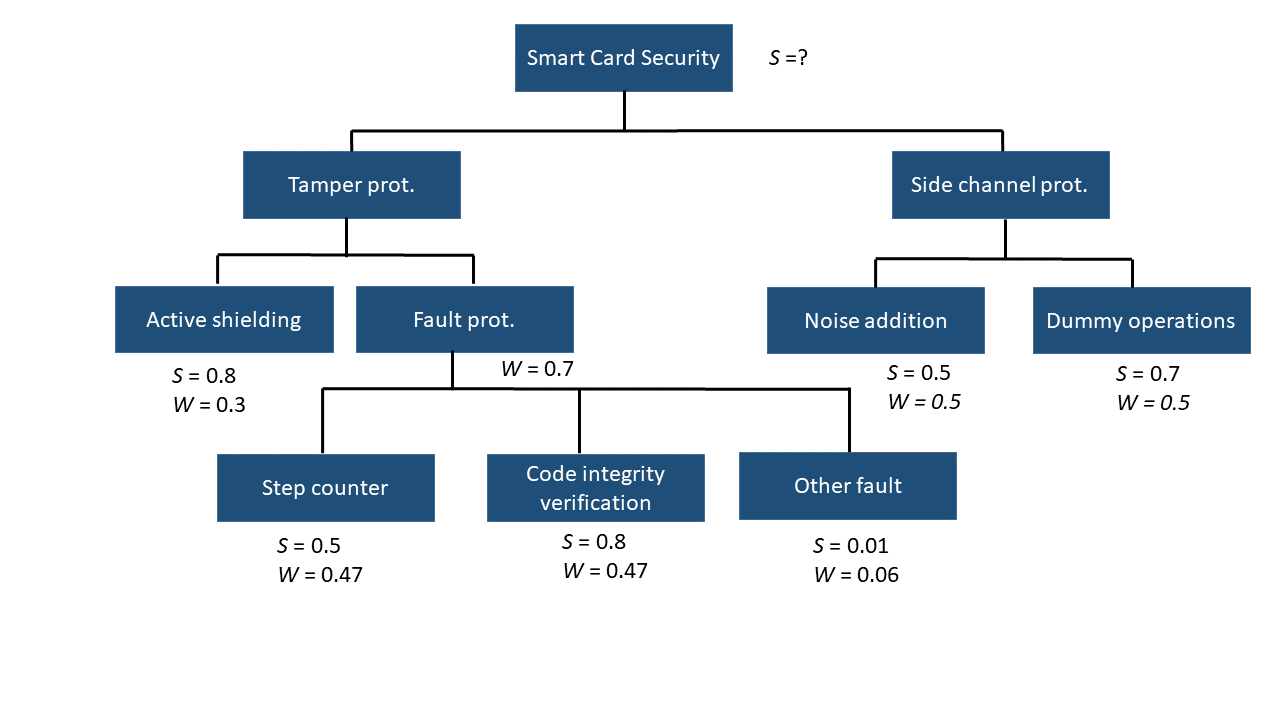
\includegraphics[scale=0.35]{./Drawings/EITP20-Secure_Systems_Engineering/Smart_Card_Security_System.png}
    \caption{Smart Card Security System}
    \label{fig:Smart_Card_Security_System}
  \end{figure}


\question{} How can the sensitivity for a certain security component be calculated?
\question{} What is a CVE database? Which organizations maintain global CVEs?
\question{} Which are the tree basic categories for which CVE scoring is based
  \begin{parts}
  \part{} Briefly explain each of the three categories and which security aspects are considered for each of them?
  \end{parts}

\question{} A communication product have three different categories of weaknesses, buffer overflow, TPM weaknesses, and authentication weakness with the CVE list below. Calculate an overall vulnerability score for the product (use the NIST CVE database to obtain the individual scores).
  \begin{parts}
  \part{} Buffer overflow: CVE--2019--2304, CVE--2019--2242, CVE--2019--10572
  \part{} TPM:\@ CVE--2019--16863, CVE--2018--6622
  \part{} Authentication: CVE--2019--3768, CVE--2019--5108,CVE--2019--17627, CVE--2018--5389
  \end{parts}

\question{} Explain the terms TOI, PP, ST and EAL used in CC evaluations.
\question{} What is the purpose with the PPs?
\question{} What is the main differences between the different EAL levels?
\end{questions}

%%% Local Variables:
%%% mode: latex
%%% TeX-master: "../EITP20-Secure_Systems_Engineering-Study_Questions"
%%% End:


\end{document}